\chapter{Some Important Points} % (fold)
\label{cha:some_important_points}
\begin{chapquote}
{C.N. Yang}
Now if we adopt the view that this arbitrary convention should be independently chosen at every space-time point, then we are naturally led to the concept of gauge fields.
\end{chapquote}

\begin{enumerate}
	\item \textbf{Difference between VBF and VBS:} From experimental point of view the difference between the two comes wheter a single boson is produced from two ($VV\rightarrow V$) or two boson is produced ($VV \rightarrow VV$). However, in principle the VBF process also alows us to seperatly study the aTGC and aQGC~\cite{Green2017}.
	\item If the broken direction in symmetry space also corresponds to a gauge symmetry (i.e. a space-time dependent symmetry) then the associated Goldstone boson and the massless gauge boson combine to form a massive gauge boson -- \textbf{the Higgs mechanism}~\cite{Chanowitz1988}.
\end{enumerate}
% chapter some_important_points (end)

\section{Weak Interaction} % (fold)
\label{sec:weak_interaction}
Initially, the weak interaction was investigated while studying the radioactivity decays of atomic nuclei. Its history is closely related with the neurtal lepton which is called neutrino by Fermi. Also, the mathematical foundation for this was developed by Fermi itself~\cite{Braibant2012}.\\
Few important points about weak interactions:
\begin{enumerate}
	\item Particles decaying through the weak interaction have relatively longer lifetimes ($\sim 10^{-10}~s$) as compared to the electromagnetic ($\sim 10^{-19}~s$) or strong interactions ($\sim 10^{-23}~s$).
	\item weak interactions do not conserve some quantum numbers, like parity $P$, the charge conjugation $C$, the strangness $S$ (with the selection rule $\Delta S = \pm 1$), that are conserved in electromagnetic or strong interaction.
	\item Weak interaction does not play any role in binding the submicroscopic atom. But it is responsible for the radioactivity $\beta$ decays, which has an important role in astrophysical systems.
	\item The weak interaction is mediated through the massive vector bosons, $W^{\pm}$ and $Z^0$, respectively with a mass of 80.3 and 91.2 GeV.
	\item The process with a $W^+$ or $W^-$ exchange are called \textbf{\textit{Charged Current interactions}}. This involves the transformation of a lepton into another lepton of the same family, like: \begin{equation}
		\bar{\nu}_{\mu} p \rightarrow \mu^+ n ~~~~(\text{High energy $\bar{\nu}_{\mu}$ interaction})
	\end{equation} or, \begin{equation}
		\bar{\nu}_{e} p \rightarrow e^+ n ~~~~(\text{High energy $\bar{\nu}_e$ interaction})
	\end{equation}
	\item The processes with a $Z^0$ exchange are called \textbf{\textit{Neutral Current interactions}}, like: \begin{equation}
		\bar{\nu}_{\mu} e^- \rightarrow \nu_{\mu} e^- ~~~~(\text{Elastic scattering})
	\end{equation} The feynman diagram illustrating both neutral current interaction and charged current interaction is shown in Fig.~\ref{fig:weak_int}.
	\item The leptonic weak vertices involve only members of same generations while in quark sector the transition between different generations are allowed.
	\item An estimate of strength of different forces can be obtained by comparing their respective lifetimes of decay involving the particles using: \begin{equation}
		\frac{\alpha_{Force-1}}{\alpha_{Force-2}} \propto \Big(\frac{\tau_{Force-1}}{\tau_{Force-2}}\Big)^{-1/2}
	\end{equation}
	where, $\alpha$ is the coupling constant for the respective interaction and $\tau$ is the lifetime of the decay.\\
	Thus,\begin{equation}
		\alpha_{strong}:\alpha_{EM}:\alpha_{weak} \propto (10^{-23})^{-1/2}:(10^{-19})^{-1/2}:(10^{-10})^{-1/2}
	\end{equation}or,
	\begin{equation}
		\alpha_{strong}:\alpha_{EM}:\alpha_{weak} \propto 10^{13/2}: 10^{9/2}: 1
	\end{equation}
\end{enumerate}



\begin{figure}[htbp]
	\centering
	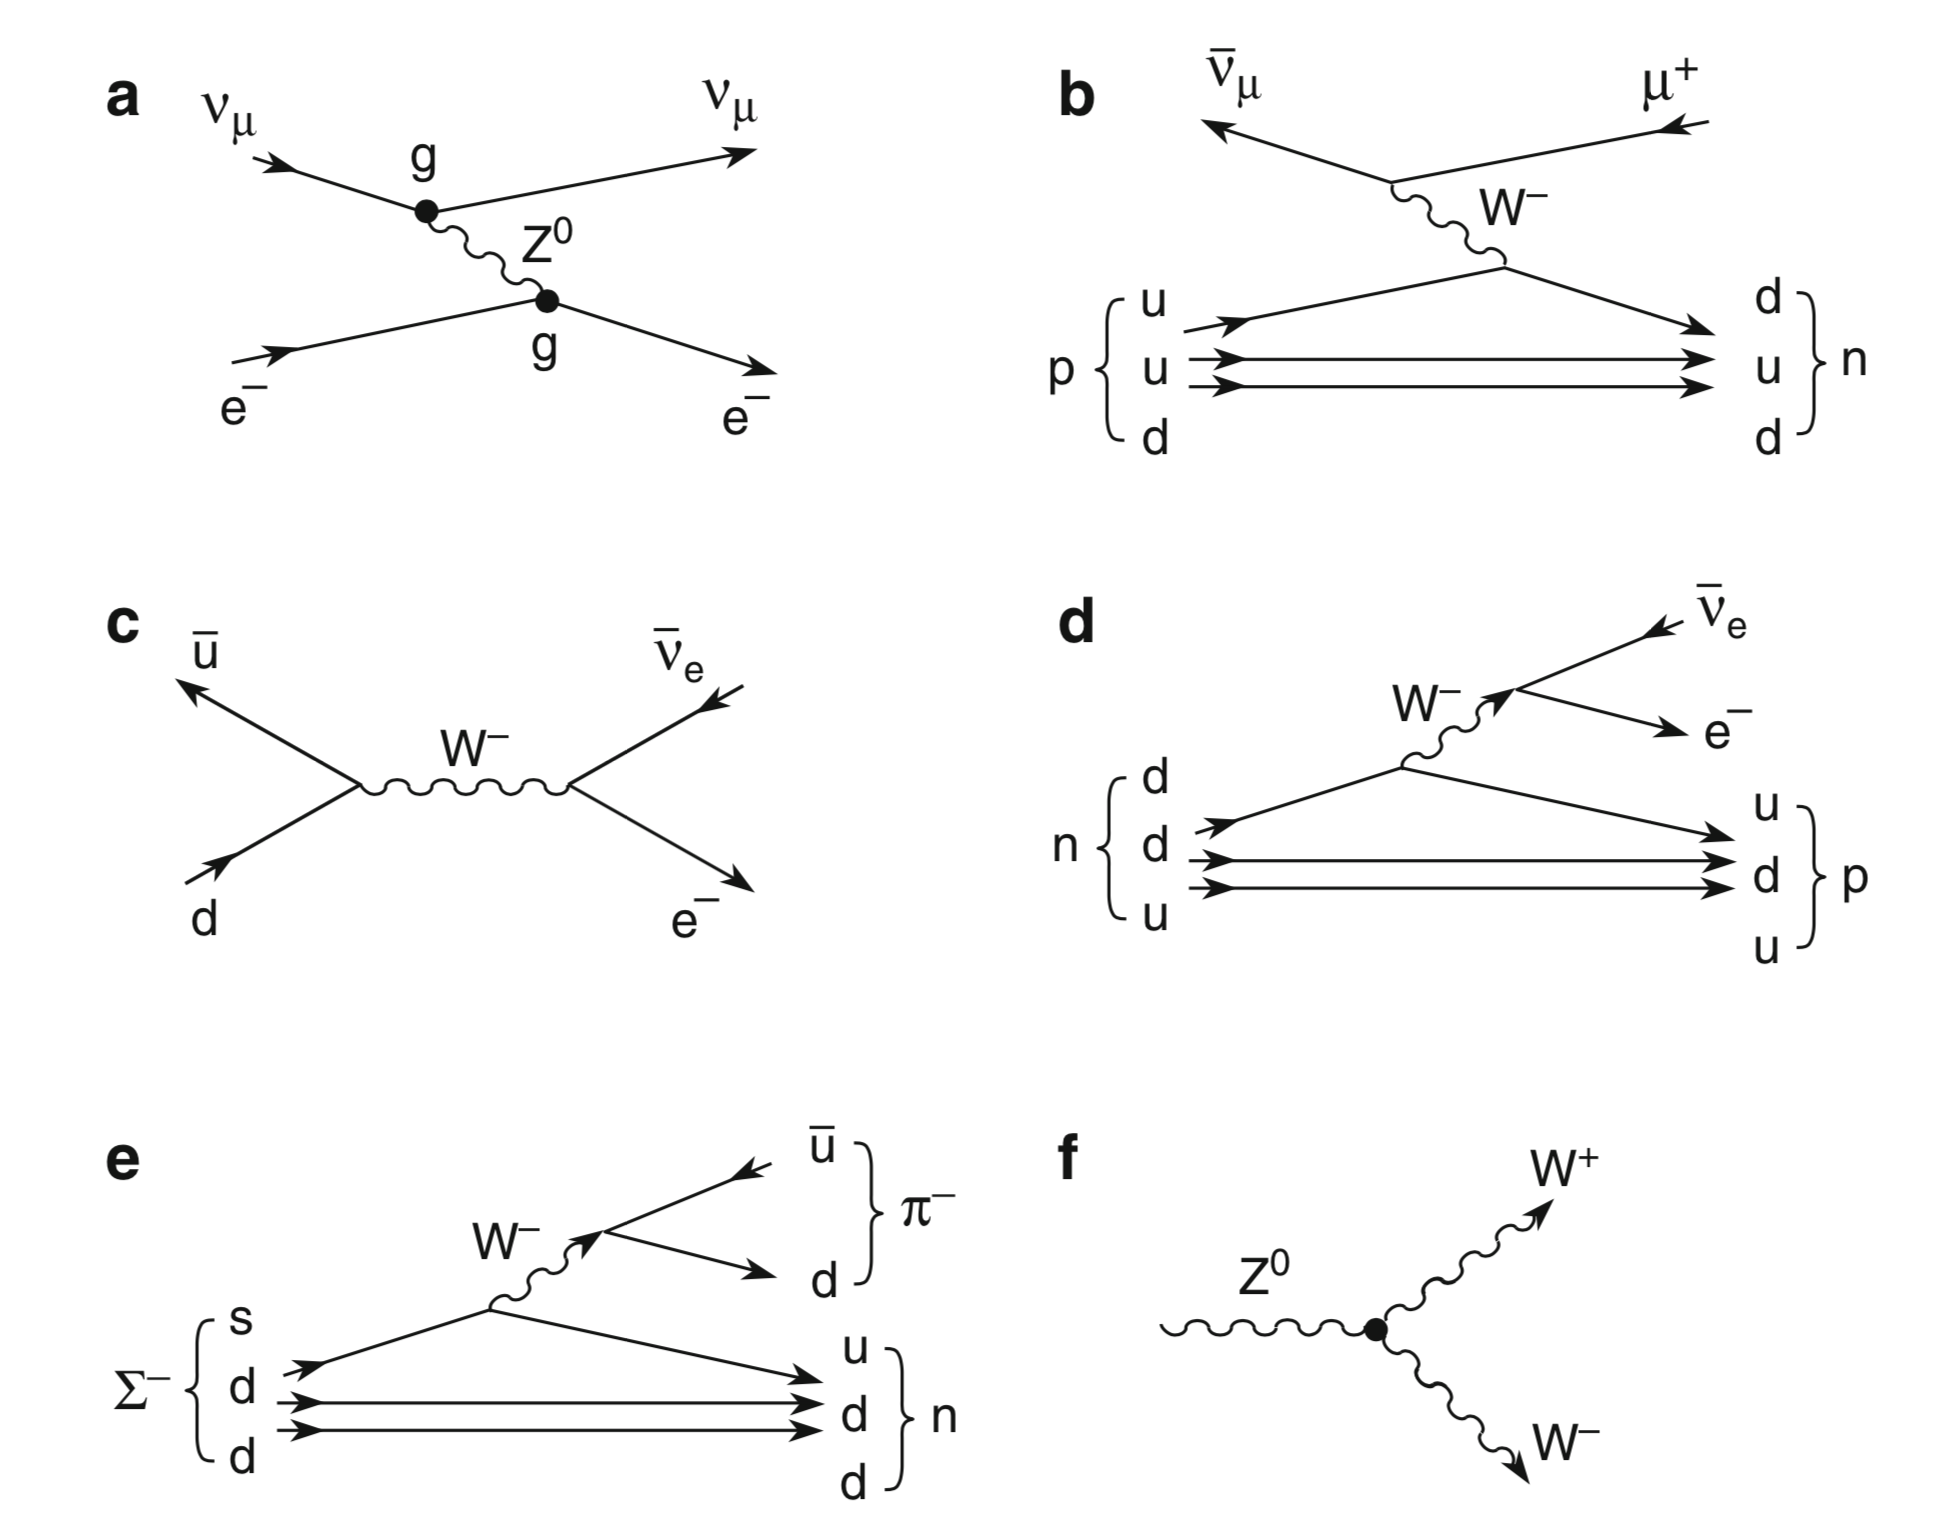
\includegraphics[width=0.95\textwidth]{figures/Intro/weak_interaction_Fey.png}
	\caption{Feynman diagram illustrating weak interaction. (a) Elasting scattering of electron and muon-neutrino and g represents the coupling constant. (b)$\bar{\nu}_{\mu} p \rightarrow \mu^+ n$ mediatead through the $W^-$ boson. (c) Charged current weak interaction involving quarks. (d) Neutron decay. (e) $\Sigma$ meason decay. (f) Triple-vertex between $Z^0$, $W^+$ and $W^-$~\cite{Braibant2012}.}
	\label{fig:weak_int}
\end{figure}

% section weak_interaction (end)